\chapter{Topology model}
\label{sec:topology_model}

In this chapter, we will describe the first component of the hierarchical topology representation, which is its topology model.

\section{Topology building blocks}
\label{sec:topology_building_blocks}
The representation system proposed in this thesis is hierarchical. This means that the system of machines can be represented using a tree structure.

The leaves in the tree are machines. Each machine has its buffer which contains jobs waiting for processing. Whenever the machine is free, a job is chosen from the buffer and put on the machine for processing.

The inner nodes in the tree are groups. Every group has at least one child component, and these components can be either machines or groups. This simple recursive rule allows building of arbitrarily complex systems of machines. Throughout the remainder of this thesis, we will refer to a system of machines and its inner connections as a topology. 

To reiterate, topologies correspond to tree structures. Another data structure which is very important for this system is directed acyclic graphs (DAGs). DAGs are used to store the possible paths which a job can take when going through the topology.

Every group can be thought of as an abstract machine. When a job enters the group, it will be processed on it, the same as it would be on a machine, but this processing will be instant and then the job will be directed to the next component on its path. There are several types of groups. 

\subsection{Serial group}

The first group type is the serial group. The components of this group are ordered. When a job enters this group, it is directed to its first component, and then second, all the way to the last one. Figure \ref{fig:serial_group} shows a serial group topology on the left, and the corresponding paths DAG on the right. Serial group nodes are named S, while machines are named M.

\begin{figure}[!htbp]
	\centering
	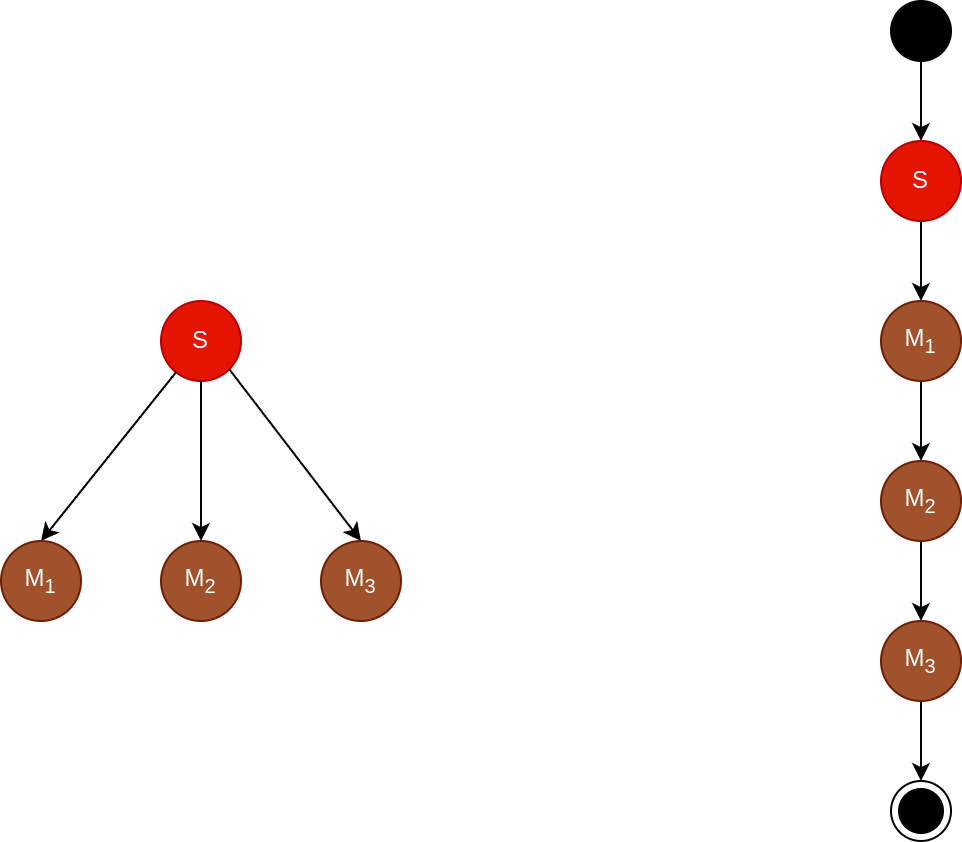
\includegraphics[scale=0.3]{../images/serial_group.png}
	\caption{Serial group - topology and paths}
    \label{fig:serial_group}
\end{figure}

\subsection{Parallel group}

The second group type is parallel group. This group performs a branching over its components. When a job enters this group, it is directed to one of its components, and the job will only be processed in that component. Figure \ref{fig:parallel_group} shows a parallel group topology on the left, and the corresponding paths DAG on the right. Parallel group nodes are named P.

\begin{figure}[!htbp]
	\centering
	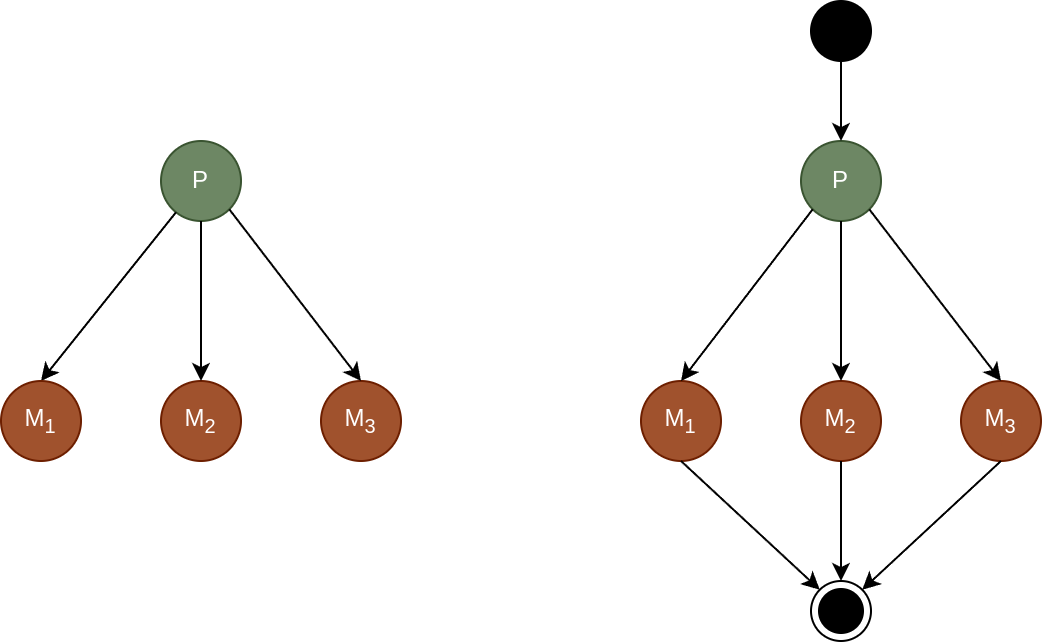
\includegraphics[scale=0.3]{../images/parallel_group.png}
	\caption{Parallel group - topology and paths}
    \label{fig:parallel_group}
\end{figure}

\subsection{Route group}

The third group type is route group. In this group, each job has a predefined route through the components of the group, and this route can differ from job to job. When a job enters this group, it is directed to the first component on its route, and then second, all the way to the last one. Figure \ref{fig:route_group} shows a route group topology on the left, and several possible paths DAGs on the right. Paths can go through all components in any order, they can contain only a subset of components, the components can be repeated in the paths, and they can even contain no components. Route group nodes are named R.

\begin{figure}[!htbp]
	\centering
	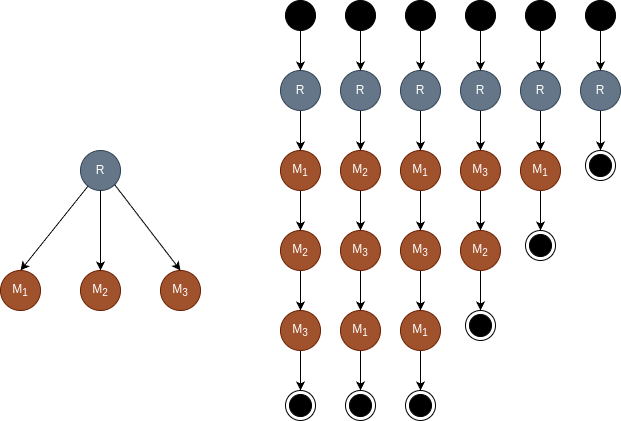
\includegraphics[scale=0.3]{../images/route_group.png}
	\caption{Route group - topology and paths}
    \label{fig:route_group}
\end{figure}

\subsection{Open group}

The fourth and the last group type is open group. In this group, each job contains a multiset of components of the group, and the job has to be processed in each component of the multiset, but it is up to the scheduler to determine the order of processing. All the same rules for paths in the route group apply here - a path can contain all components, it can contain some components, components can be repeated, and it can contain no components. Figure \ref{fig:open_group} shows an open group topology on the left, and several possible paths DAGs on the right. Open group nodes are named O. The DAG notation is expanded here to be able to represent open groups. In each path, all the components of open groups are connected to it by dashed lines. When the job arrives at an open group node, it has to go through all its components in any order, and then it proceeds to the next node in the path.

\begin{figure}[!htbp]
	\centering
	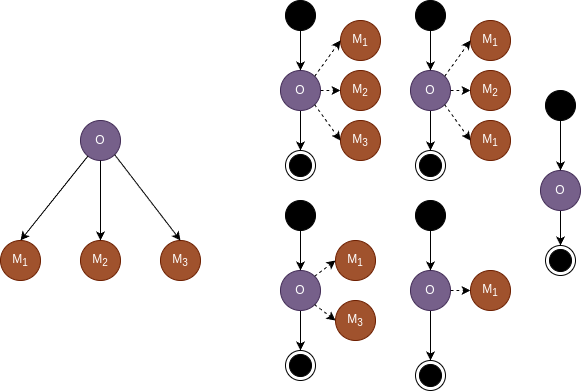
\includegraphics[scale=0.3]{../images/open_group.png}
	\caption{Open group - topology and paths}
    \label{fig:open_group}
\end{figure}

\section{Machine environments}
\label{sec:machine_environments}
The scheduling model described in \citep{pinedo2016scheduling} defines several machine environments. Here, we will go over each one of them, and describe how they can be implemented using the hierarchical topology representation. In other words, here we will describe how our topology model handles $\alpha$ entries from the scheduling problem definition.

The first environment is $1$ (single machine). This can be very easily achieved using a topology that contains a single machine element.

Several environments can be achieved using a parallel group topology element. These are $P_m$ (identical machines in parallel), $Q_m$ (machines of different speeds in parallel) and $R_m$ (unrelated machines in parallel). Machines and jobs can be divided into several types, and we can define the processing time for each combination of machine type and job type.

The machine environment $F_m$ (flow shop) can be achieved using a serial group topology element.

The machine environment $FF_c$ (flexible flow shop) consists of $c$ stages in series, where each stage contains a number of machines in parallel. Figure \ref{fig:flexible_flow_shop} shows how this environment can be achieved, with topology at the top and paths DAG at the bottom.

\begin{figure}[!htbp]
	\centering
	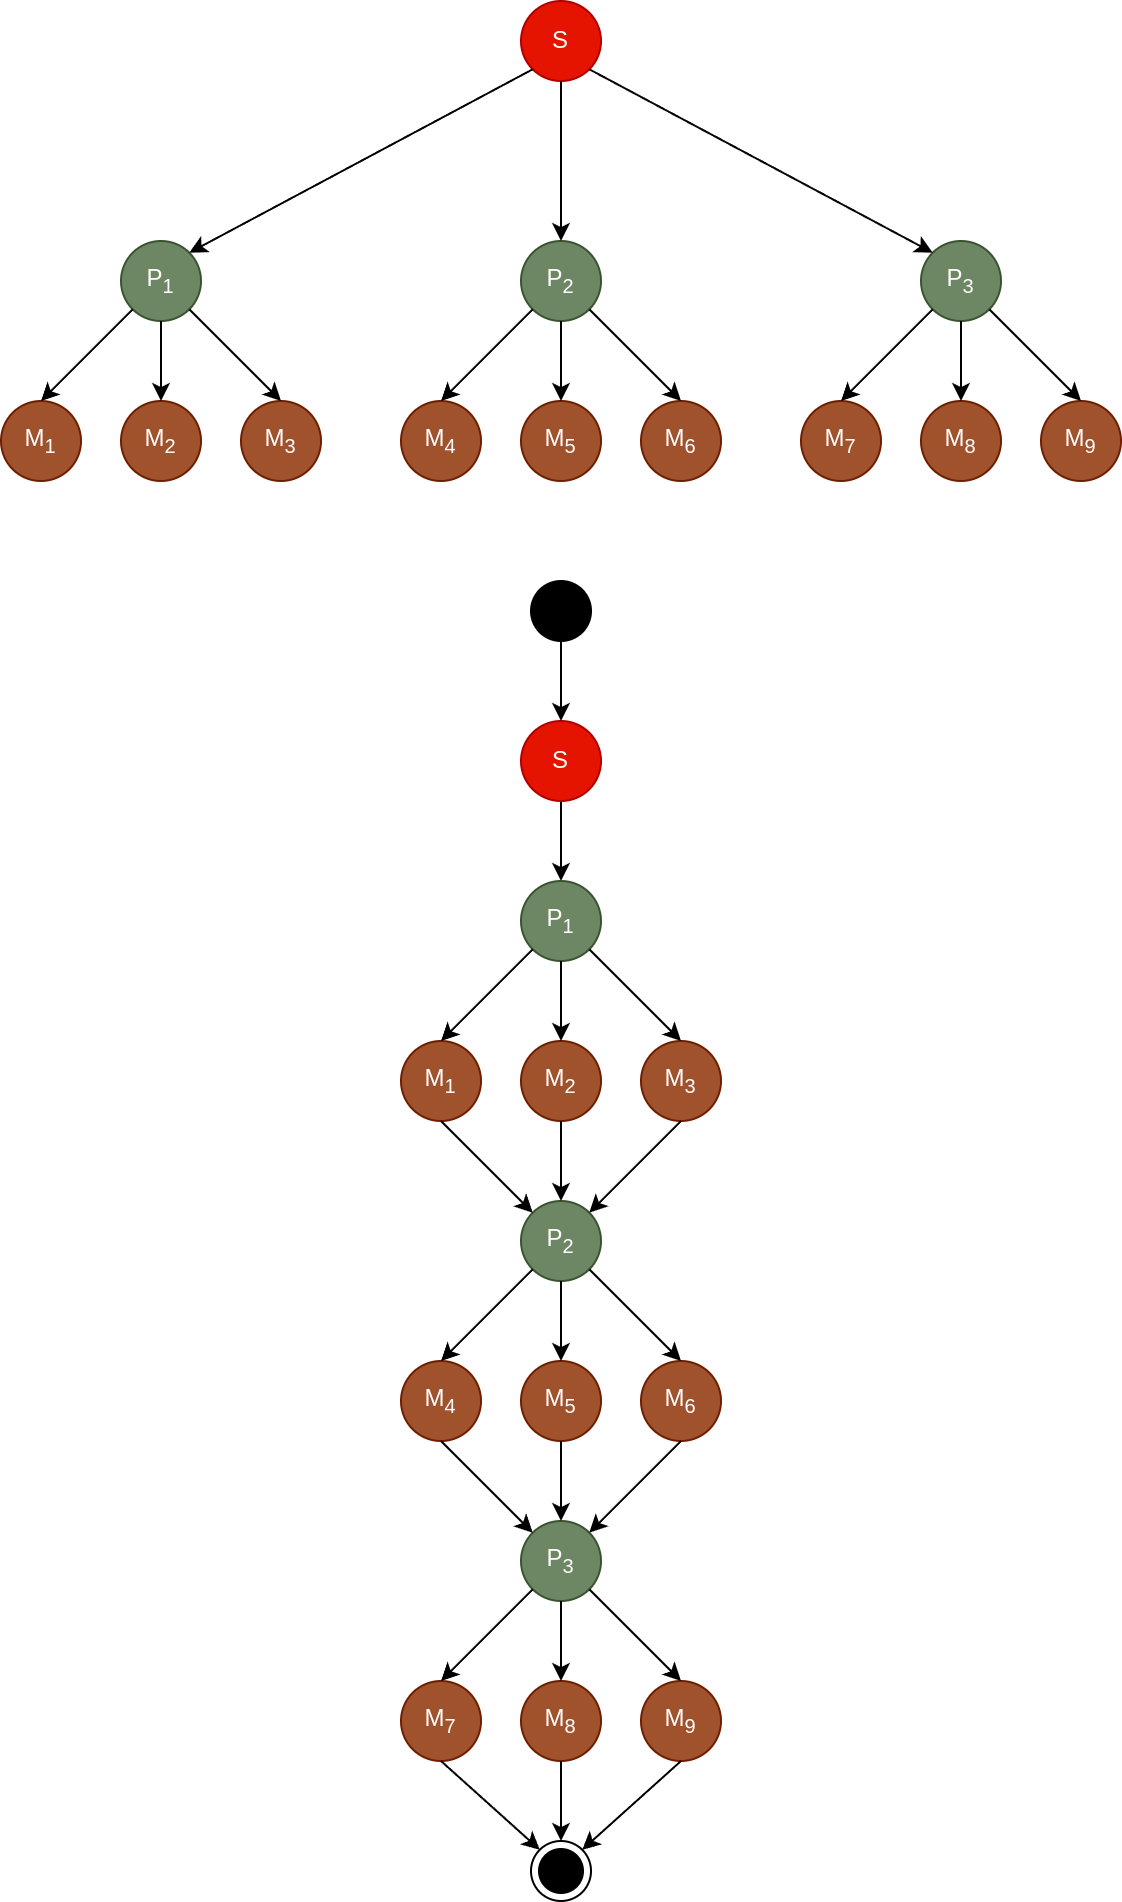
\includegraphics[scale=0.3]{../images/flexible_flow_shop.png}
	\caption{Flexible flow shop - topology and paths}
    \label{fig:flexible_flow_shop}
\end{figure}

The machine environment $J_m$ (job shop) consists of several machines, and each job has its own predetermined route through the machines of the job shop. This environment can be achieved using a route group topology element.

The machine environment $FJ_c$ (flexible job shop) consists of $c$ stages, and each stage contains several machines in parallel. Each job has its predetermined route through the system, and at every stage any machine in parallel can process the job. Figure \ref{fig:flexible_job_shop} shows one way to achieve this environment, with topology at the top and several possible paths DAGs at the bottom.

\begin{figure}[!htbp]
	\centering
	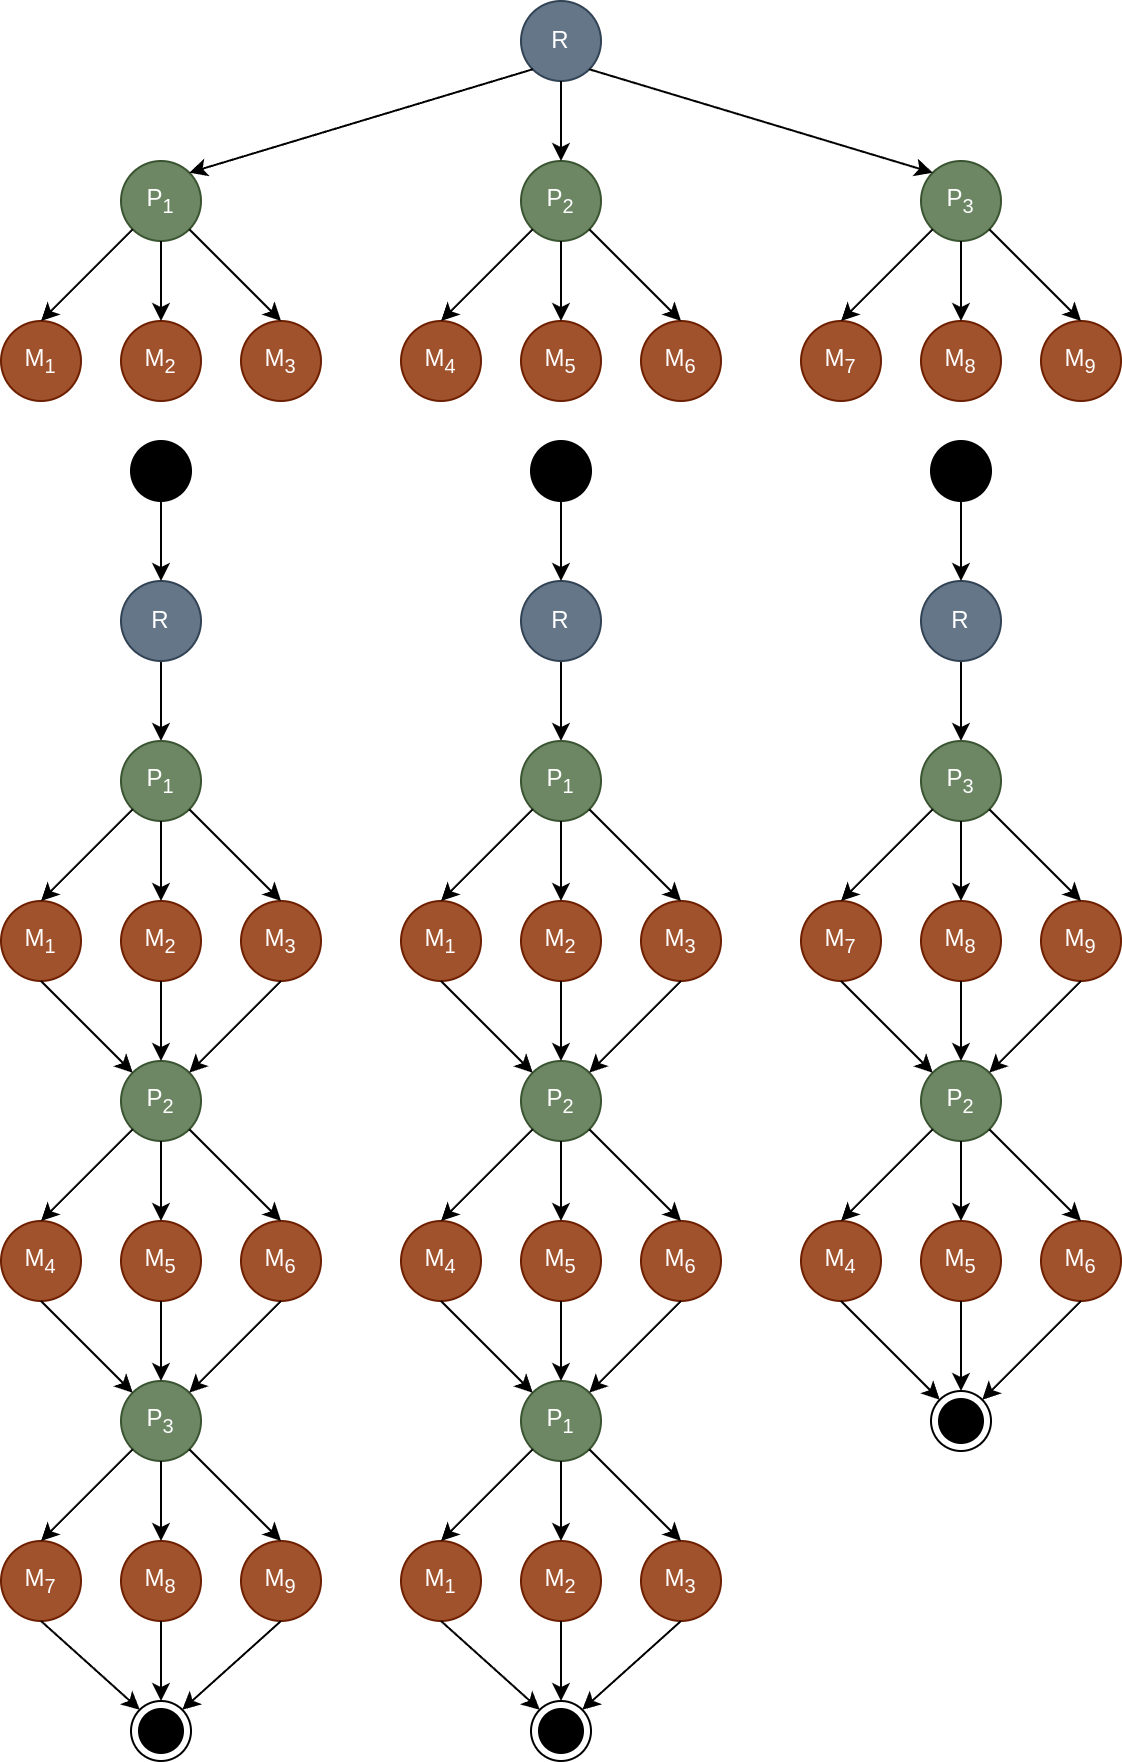
\includegraphics[scale=0.3]{../images/flexible_job_shop.png}
	\caption{Flexible job shop - topology and paths}
    \label{fig:flexible_job_shop}
\end{figure}

Finally, the machine environment $O_m$ (open machines) consists of $m$ machines, where each job has to be processed on each machine, but there are no restrictions regarding the routing of the job, and it is up to the scheduler to determine a route for each job. This environment can be achieved using an open group topology element.

As we have demonstrated, the hierarchical topology representation is a very versatile representation system. It is capable of implementing all the standard types of machine environments, but it can also implement environments which are much more complex, due to its capabilities being defined by recursive rules.